


%% need no \usepackage{Sweave.sty}



%





%% use JSS class -- use 'nojss' to turn off header
\documentclass[shortnames,nojss,article]{jss}\usepackage{graphicx, color}
%% maxwidth is the original width if it is less than linewidth
%% otherwise use linewidth (to make sure the graphics do not exceed the margin)
\makeatletter
\def\maxwidth{ %
  \ifdim\Gin@nat@width>\linewidth
    \linewidth
  \else
    \Gin@nat@width
  \fi
}
\makeatother

\definecolor{fgcolor}{rgb}{0.2, 0.2, 0.2}
\newcommand{\hlnumber}[1]{\textcolor[rgb]{0,0,0}{#1}}%
\newcommand{\hlfunctioncall}[1]{\textcolor[rgb]{0.501960784313725,0,0.329411764705882}{\textbf{#1}}}%
\newcommand{\hlstring}[1]{\textcolor[rgb]{0.6,0.6,1}{#1}}%
\newcommand{\hlkeyword}[1]{\textcolor[rgb]{0,0,0}{\textbf{#1}}}%
\newcommand{\hlargument}[1]{\textcolor[rgb]{0.690196078431373,0.250980392156863,0.0196078431372549}{#1}}%
\newcommand{\hlcomment}[1]{\textcolor[rgb]{0.180392156862745,0.6,0.341176470588235}{#1}}%
\newcommand{\hlroxygencomment}[1]{\textcolor[rgb]{0.43921568627451,0.47843137254902,0.701960784313725}{#1}}%
\newcommand{\hlformalargs}[1]{\textcolor[rgb]{0.690196078431373,0.250980392156863,0.0196078431372549}{#1}}%
\newcommand{\hleqformalargs}[1]{\textcolor[rgb]{0.690196078431373,0.250980392156863,0.0196078431372549}{#1}}%
\newcommand{\hlassignement}[1]{\textcolor[rgb]{0,0,0}{\textbf{#1}}}%
\newcommand{\hlpackage}[1]{\textcolor[rgb]{0.588235294117647,0.709803921568627,0.145098039215686}{#1}}%
\newcommand{\hlslot}[1]{\textit{#1}}%
\newcommand{\hlsymbol}[1]{\textcolor[rgb]{0,0,0}{#1}}%
\newcommand{\hlprompt}[1]{\textcolor[rgb]{0.2,0.2,0.2}{#1}}%

\usepackage{framed}
\makeatletter
\newenvironment{kframe}{%
 \def\at@end@of@kframe{}%
 \ifinner\ifhmode%
  \def\at@end@of@kframe{\end{minipage}}%
  \begin{minipage}{\columnwidth}%
 \fi\fi%
 \def\FrameCommand##1{\hskip\@totalleftmargin \hskip-\fboxsep
 \colorbox{shadecolor}{##1}\hskip-\fboxsep
     % There is no \\@totalrightmargin, so:
     \hskip-\linewidth \hskip-\@totalleftmargin \hskip\columnwidth}%
 \MakeFramed {\advance\hsize-\width
   \@totalleftmargin\z@ \linewidth\hsize
   \@setminipage}}%
 {\par\unskip\endMakeFramed%
 \at@end@of@kframe}
\makeatother

\definecolor{shadecolor}{rgb}{.97, .97, .97}
\definecolor{messagecolor}{rgb}{0, 0, 0}
\definecolor{warningcolor}{rgb}{1, 0, 1}
\definecolor{errorcolor}{rgb}{1, 0, 0}
\newenvironment{knitrout}{}{} % an empty environment to be redefined in TeX

\usepackage{alltt}
\usepackage{booktabs,flafter,thumbpdf}
%\VignetteIndexEntry{An Introduction to dendextend}
%\VignetteKeywords{Dendrogram, hclust, heirarchical clustering, visualization, tanglegram, R}
%\VignettePackage{dendextend}
%\VignetteEngine{knitr::knitr}


\author{Tal Galili\\Tel-Aviv University \And Yoav Benjamini\\Tel-Aviv University}
\Plainauthor{Tal Galili, Yoav Benjamini}




% \Plaintitle{Doing More with Dendrograms: The dendextend R Package}
% \title{Doing More with Dendrograms:\\ The \pkg{dendextend} \proglang{R} Package}

\Plaintitle{Comparing and Manipulating Dendrograms: The dendextend R Package}
\title{Comparing and Manipulating Dendrograms:\\ The \pkg{dendextend} \proglang{R} Package}


\Abstract{
The \pkg{dendextend} package extends the dendrogram objects in \proglang{R}.

The paper gives a detailed exposition of both the internal structure of
the package and the provided user interfaces.
}

\Keywords{Dendrogram, hclust, hierarchical clustering, visualization, tanglegram,  \proglang{R}}
\Plainkeywords{Dendrogram, hclust, hierarchical clustering, visualization, tanglegram, R}


% \Volume{40}
% \Issue{8}
% \Month{April}
% \Year{2011}
% \Submitdate{2010-11-15}
% \Acceptdate{2011-03-21}

\Address{
  Tal Galili \\
   Department of Statistics and Operations Research \\
   Tel Aviv University, Israel \\
   E-mail: \email{tal.galili@math.tau.ac.il}\\
   URLs: \url{http://www.r-statistics.com/}, 
         \url{http://www.r-bloggers.com/}\\

  Yoav Benjamini\\
   The Nathan and Lily Silver\\
   Professor of Applied Statistics\\
   Department of Statistics and Operations Research \\
   Tel Aviv University, Israel \\
   E-mail: \email{ybenja@tau.ac.il}\\
   URL: \url{http://www.tau.ac.il/~ybenja/}
}
\IfFileExists{upquote.sty}{\usepackage{upquote}}{}



\begin{document}
\vspace*{-0.25cm}

%% Doesn't seem to work:
%% \tableofcontents


\section{Introduction}

\subsection{The \code{dendrogram} object}

The \code{dendrogram} class provides general functions for handling tree-like structures in \proglang{R} \citep{R:Main}. It is intended as a replacement for similar functions in hierarchical clustering and classification/regression trees, such that all of these can use the same engine for plotting or cutting trees.

A dendrogram object represents a tree as a nested \code{list} object, with various attributes.

Dendrogram has several useful methods bundled with R:

\begin{knitrout}
\definecolor{shadecolor}{rgb}{0.969, 0.969, 0.969}\color{fgcolor}\begin{kframe}
\begin{alltt}
\hlfunctioncall{methods}(class = \hlstring{"dendrogram"})
\end{alltt}
\begin{verbatim}
##  [1] [[.dendrogram*         as.hclust.dendrogram*  cophenetic.dendrogram*
##  [4] cut.dendrogram*        head.dendrogram*       labels.dendrogram*    
##  [7] labels<-.dendrogram*   merge.dendrogram*      nleaves.dendrogram*   
## [10] plot.dendrogram*       print.dendrogram*      reorder.dendrogram*   
## [13] rev.dendrogram*        rotate.dendrogram*     sort.dendrogram*      
## [16] str.dendrogram*        trim.dendrogram*       unroot.dendrogram*    
## 
##    Non-visible functions are asterisked
\end{verbatim}
\end{kframe}
\end{knitrout}


For example, let's create a dendrogram object based on an hierarchical clustering of 4 states in the U.S.:

\begin{knitrout}
\definecolor{shadecolor}{rgb}{0.969, 0.969, 0.969}\color{fgcolor}\begin{kframe}
\begin{alltt}
\hlcomment{# our data:}
\hlfunctioncall{data}(USArrests)
US_data <- USArrests[\hlfunctioncall{c}(2, 5, 32, 35), ]
\hlfunctioncall{print}(US_data)
\end{alltt}
\begin{verbatim}
##            Murder Assault UrbanPop Rape
## Alaska       10.0     263       48 44.5
## California    9.0     276       91 40.6
## New York     11.1     254       86 26.1
## Ohio          7.3     120       75 21.4
\end{verbatim}
\begin{alltt}

hc <- \hlfunctioncall{hclust}(\hlfunctioncall{dist}(US_data), \hlstring{"ave"})  # create an heirarchical clustering object
dend <- \hlfunctioncall{as.dendrogram}(hc)
\end{alltt}
\end{kframe}
\end{knitrout}



Below are examples for some dendrogram methods:

\begin{knitrout}
\definecolor{shadecolor}{rgb}{0.969, 0.969, 0.969}\color{fgcolor}\begin{kframe}
\begin{alltt}
\hlfunctioncall{print}(dend)
\end{alltt}
\begin{verbatim}
## 'dendrogram' with 2 branches and 4 members total, at height 146.7
\end{verbatim}
\begin{alltt}
\hlfunctioncall{labels}(dend)
\end{alltt}
\begin{verbatim}
## [1] "Ohio"       "Alaska"     "California" "New York"
\end{verbatim}
\begin{alltt}
\hlfunctioncall{str}(dend)
\end{alltt}
\begin{verbatim}
## --[dendrogram w/ 2 branches and 4 members at h = 147]
##   |--leaf "Ohio" 
##   `--[dendrogram w/ 2 branches and 3 members at h = 44.1]
##      |--leaf "Alaska" 
##      `--[dendrogram w/ 2 branches and 2 members at h = 26.9]
##         |--leaf "California" 
##         `--leaf "New York"
\end{verbatim}
\begin{alltt}
\hlfunctioncall{str}(dend[[2]])  \hlcomment{# looking at one branch of the dendrogram}
\end{alltt}
\begin{verbatim}
## --[dendrogram w/ 2 branches and 3 members at h = 44.1]
##   |--leaf "Alaska" 
##   `--[dendrogram w/ 2 branches and 2 members at h = 26.9]
##      |--leaf "California" 
##      `--leaf "New York"
\end{verbatim}
\begin{alltt}
\hlfunctioncall{plot}(dend)
\end{alltt}
\end{kframe}

{\centering 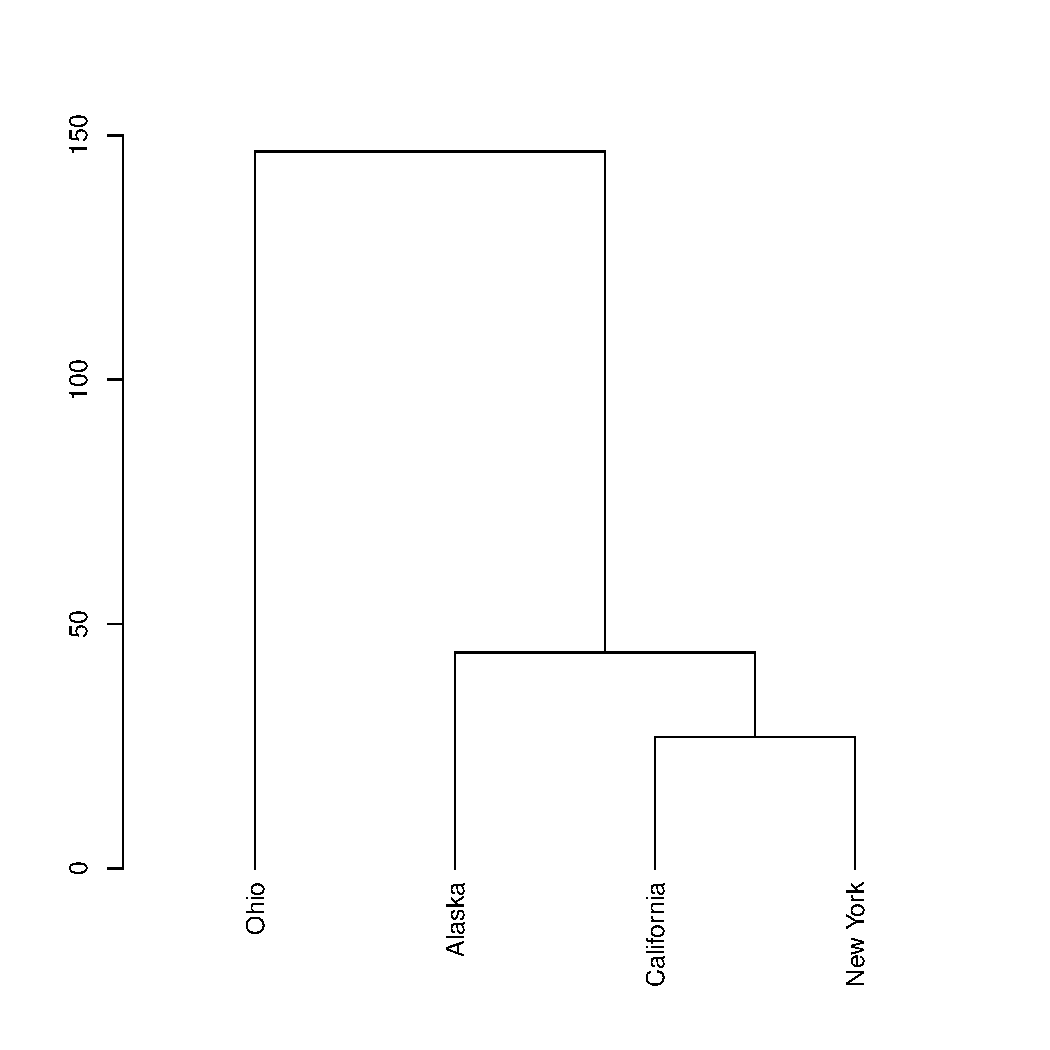
\includegraphics[width=4in,height=4in]{figure/unnamed-chunk-4} 

}



\end{knitrout}


You might notice how the order of the items (leaves/terminal nodes) of the dendrogram is different than their order in the table. In order to re-order the rows in the data-table to have the same order as the items in the dendrogram, we can use the \code{order.dendrogram} function:

\begin{knitrout}
\definecolor{shadecolor}{rgb}{0.969, 0.969, 0.969}\color{fgcolor}\begin{kframe}
\begin{alltt}
(new_order <- \hlfunctioncall{order.dendrogram}(dend))
\end{alltt}
\begin{verbatim}
## [1] 4 1 2 3
\end{verbatim}
\begin{alltt}
\hlcomment{# the order of the original items to have them be at the same order as}
\hlcomment{# they assume in the dendrogram}
\hlfunctioncall{print}(US_data[new_order, ])
\end{alltt}
\begin{verbatim}
##            Murder Assault UrbanPop Rape
## Ohio          7.3     120       75 21.4
## Alaska       10.0     263       48 44.5
## California    9.0     276       91 40.6
## New York     11.1     254       86 26.1
\end{verbatim}
\end{kframe}
\end{knitrout}



In order to see what our dendrogram (\code{list}) object includes, we need to use the \code{unclass} function, which will strip away the class attribute and will allow us to print the list as is, without going through the \code{print.dendrogram} method. We can see how each node in the dendrogram/list object has the following (self explaining) attributes:

\begin{knitrout}
\definecolor{shadecolor}{rgb}{0.969, 0.969, 0.969}\color{fgcolor}\begin{kframe}
\begin{alltt}
\hlfunctioncall{str}(\hlfunctioncall{unclass}(dend))
\end{alltt}
\begin{verbatim}
## List of 2
##  $ : atomic [1:1] 4
##   ..- attr(*, "members")= int 1
##   ..- attr(*, "height")= num 0
##   ..- attr(*, "label")= chr "Ohio"
##   ..- attr(*, "leaf")= logi TRUE
##  $ :List of 2
##   ..$ : atomic [1:1] 1
##   .. ..- attr(*, "members")= int 1
##   .. ..- attr(*, "height")= num 0
##   .. ..- attr(*, "label")= chr "Alaska"
##   .. ..- attr(*, "leaf")= logi TRUE
##   ..$ :List of 2
##   .. ..$ : atomic [1:1] 2
##   .. .. ..- attr(*, "label")= chr "California"
##   .. .. ..- attr(*, "members")= int 1
##   .. .. ..- attr(*, "height")= num 0
##   .. .. ..- attr(*, "leaf")= logi TRUE
##   .. ..$ : atomic [1:1] 3
##   .. .. ..- attr(*, "label")= chr "New York"
##   .. .. ..- attr(*, "members")= int 1
##   .. .. ..- attr(*, "height")= num 0
##   .. .. ..- attr(*, "leaf")= logi TRUE
##   .. ..- attr(*, "members")= int 2
##   .. ..- attr(*, "midpoint")= num 0.5
##   .. ..- attr(*, "height")= num 26.9
##   ..- attr(*, "members")= int 3
##   ..- attr(*, "midpoint")= num 0.75
##   ..- attr(*, "height")= num 44.1
##  - attr(*, "members")= int 4
##  - attr(*, "midpoint")= num 0.875
##  - attr(*, "height")= num 147
\end{verbatim}
\end{kframe}
\end{knitrout}



Notice how terminal nodes uses the "leaf" attribute (set to TRUE).
\begin{knitrout}
\definecolor{shadecolor}{rgb}{0.969, 0.969, 0.969}\color{fgcolor}\begin{kframe}
\begin{alltt}
\hlfunctioncall{names}(\hlfunctioncall{attributes}(dend)[-4])
\end{alltt}
\begin{verbatim}
## [1] "members"  "midpoint" "height"
\end{verbatim}
\end{kframe}
\end{knitrout}




A very important function is \code{dendrapply}. It applies some function recursively to each node of a dendrogram. It is often used for adjusting attributes of the object, or extracting something from it. 

One current "feature" with this function is that just sending a dendrogram through it will return it with each of its nodes becoming of class "dendrogram". Notice the use of the \code{unclass_dend} function. Example:

\begin{knitrout}
\definecolor{shadecolor}{rgb}{0.969, 0.969, 0.969}\color{fgcolor}\begin{kframe}
\begin{alltt}
\hlcomment{# dendrapply(dend, unclass) # in case the}
itself <- \hlfunctioncall{function}(x) x
dend_from_dendrapply <- \hlfunctioncall{dendrapply}(dend, itself)

\hlcomment{# here we must first use unclass since '[[]]' inherits its class to the}
\hlcomment{# output:}
\hlfunctioncall{class}(\hlfunctioncall{unclass}(dend)[[2]])
\end{alltt}
\begin{verbatim}
## [1] "list"
\end{verbatim}
\begin{alltt}
\hlfunctioncall{class}(\hlfunctioncall{unclass}(dend_from_dendrapply)[[2]])
\end{alltt}
\begin{verbatim}
## [1] "dendrogram"
\end{verbatim}
\begin{alltt}
\hlfunctioncall{class}(\hlfunctioncall{unclass_dend}(dend_from_dendrapply)[[2]])  \hlcomment{# the new uncless_dend solves it.}
\end{alltt}
\begin{verbatim}
## [1] "list"
\end{verbatim}
\end{kframe}
\end{knitrout}




\subsection{Motivation for creating \code{dendextend}}



The \code{dendrogram} object has several \textbf{advantages}:

\begin{enumerate}

   \item \code{dendrogram} objects are list R objects. This makes their structure very familiar and easy to understand by R users. They are also, relatively, simple to manipulate and extend.
   \item \code{dendrogram} objects has various methods and functions for using them within R base. 
   \item Other tree objects, such as \code{hclust}, and objects from the \pkg{ape} package \citep{CRAN:ape},  include an \code{as.dendrogram} method for converting their objects into a dendrogram. And also \code{as.phylo.dendrogram}, \code{as.hclust.dendrogram}.
   \item \code{dendrogram} objects are used in various packages as an intermediate step for other purposes (often plotting), such as:
   
   \begin{enumerate}
   \item The \pkg{latticeExtra} package \citep{CRAN:latticeExtra}, see the \code{dendrogramGrob} function.
   \item The \pkg{labeltodendro} package \citep{CRAN:labeltodendro}, see the \code{colorplot} function.
   \item The \pkg{bclust} package \citep{CRAN:bclust}, see the \code{bclust} function.
   \item The \pkg{ggdendro} package \citep{CRAN:ggdendro}, see the \code{dendro_data} function.
   \item The \pkg{Heatplus} package \citep{CRAN:Heatplus}, see the \code{annHeatmap2} function.
   \item The \pkg{sparcl} package \citep{CRAN:Heatplus}, see the \code{ColorDendrogram} function.
   \end{enumerate}
   
\end{enumerate}
   
   %\pkg{DendSer} (see the \code{} function), 


However, even with all of its advantages, the \code{dendrogram} class in R still lacks various basic features.

The \code{dendextend} package aims at filling some gaps in base R, by extending the available functions for dendrogram manipulation, statistical analysis, and visualization.

This vignettes Provides a step-by-step description of the functionality provided by the \code{dendextend} package.


\subsection{Installing \code{dendextend}}

To install the stable version from CRAN use:

\begin{knitrout}
\definecolor{shadecolor}{rgb}{0.969, 0.969, 0.969}\color{fgcolor}\begin{kframe}
\begin{alltt}
\hlfunctioncall{install.packages}(\hlstring{"dendextend"})  # not yet available from CRAN
\end{alltt}
\end{kframe}
\end{knitrout}



To install the \href{https://github.com/talgalili/dendextend}{GitHub version} use:

\begin{knitrout}
\definecolor{shadecolor}{rgb}{0.969, 0.969, 0.969}\color{fgcolor}\begin{kframe}
\begin{alltt}
\hlfunctioncall{if} (!\hlfunctioncall{require}(\hlstring{"devtools"})) \hlfunctioncall{install.packages}(\hlstring{"devtools"})
\hlfunctioncall{require}(\hlstring{"devtools"})
\hlfunctioncall{install_github}(\hlstring{"dendextend"}, \hlstring{"talgalili"})
\end{alltt}
\end{kframe}
\end{knitrout}



\section{Tree labels (extraction, assignment, length)}


\subsection{labels in base R}

In base R, the \code{labels} function is intended to find/extract a suitable set of labels from an object for use in printing or plotting, for example. By default, it uses the \code{names} and \code{dimnames} functions.

What base R \code{labels} function is missing is assignment. In the next few examples we will go through different examples of what the \code{dendextend} package offers for various objects.

\textbf{Credits:} These assignment functions were originally written by Gavin Simpson (in a post on \href{http://stackoverflow.com/questions/4614223/how-to-have-the-following-work-labelsx-some-value-r-question}{(stackoverflow)}), and adopted/adjusted to this package by Tal Galili. Some modification were inspired by Gregory Jefferis's code from the \pkg{dendroextras} package.


\subsection{labels for vectors and matrices}

In base R, for vectors, labels gives the \code{names} of the object. And if these are missing, then \code{labels} will give the vector itself as a character vector:

\begin{knitrout}
\definecolor{shadecolor}{rgb}{0.969, 0.969, 0.969}\color{fgcolor}\begin{kframe}
\begin{alltt}
x <- 1:3
\hlfunctioncall{names}(x)  \hlcomment{# this vector has no names}
\end{alltt}
\begin{verbatim}
## NULL
\end{verbatim}
\begin{alltt}
\hlfunctioncall{labels}(x)  \hlcomment{# this vector has no labels}
\end{alltt}
\begin{verbatim}
## [1] "1" "2" "3"
\end{verbatim}
\end{kframe}
\end{knitrout}


Assignment to names is available in base R and works as follows:

\begin{knitrout}
\definecolor{shadecolor}{rgb}{0.969, 0.969, 0.969}\color{fgcolor}\begin{kframe}
\begin{alltt}
x <- 1:3
\hlfunctioncall{names}(x) <- letters[1:3]  \hlcomment{# assignment for names is in base R}
\hlcomment{# both names and labels will give the same result:}
\hlfunctioncall{names}(x)
\end{alltt}
\begin{verbatim}
## [1] "a" "b" "c"
\end{verbatim}
\begin{alltt}
\hlfunctioncall{labels}(x)
\end{alltt}
\begin{verbatim}
## [1] "a" "b" "c"
\end{verbatim}
\end{kframe}
\end{knitrout}



The new labels assignment function will allow a user to change the labels of the vector just as if it was "names":

\begin{knitrout}
\definecolor{shadecolor}{rgb}{0.969, 0.969, 0.969}\color{fgcolor}\begin{kframe}
\begin{alltt}
x <- 1:3
\hlfunctioncall{labels}(x) <- letters[1:3]
\hlfunctioncall{names}(x)
\end{alltt}
\begin{verbatim}
## [1] "a" "b" "c"
\end{verbatim}
\begin{alltt}
\hlfunctioncall{labels}(x)
\end{alltt}
\begin{verbatim}
## [1] "a" "b" "c"
\end{verbatim}
\end{kframe}
\end{knitrout}


Labels assignment are also available for matrices.


\subsection{labels for dendrogram objects}

We can get a dendrogram's labels using the \code{labels} function from base R. However, in order to assign new values to it, we'll need the assignment function from \pkg{dendextend}:

\begin{knitrout}
\definecolor{shadecolor}{rgb}{0.969, 0.969, 0.969}\color{fgcolor}\begin{kframe}
\begin{alltt}
\hlfunctioncall{labels}(dend)  \hlcomment{# from base R}
\end{alltt}
\begin{verbatim}
## [1] "Ohio"       "Alaska"     "California" "New York"
\end{verbatim}
\begin{alltt}
\hlfunctioncall{set.seed}(2354235)
\hlfunctioncall{labels}(dend) <- \hlfunctioncall{sample}(\hlfunctioncall{labels}(dend))  \hlcomment{# labels assingment - thanks to dendextend}
\hlfunctioncall{labels}(dend)
\end{alltt}
\begin{verbatim}
## [1] "New York"   "Ohio"       "Alaska"     "California"
\end{verbatim}
\end{kframe}
\end{knitrout}



\subsection{labels for hclust objects}

\pkg{dendextend} offers a \code{labels} method for \code{hclust} objects. It take special care to have the order of the labels be the same as is with dendrogram object, which is the order of the labels in the plotted tree. This can be turned off when using the \code{order} parameter:

\begin{knitrout}
\definecolor{shadecolor}{rgb}{0.969, 0.969, 0.969}\color{fgcolor}\begin{kframe}
\begin{alltt}
\hlcomment{# All are from dendextend}
\hlfunctioncall{labels}(hc)
\end{alltt}
\begin{verbatim}
## [1] "Ohio"       "Alaska"     "California" "New York"
\end{verbatim}
\begin{alltt}
\hlfunctioncall{labels}(hc, order = FALSE)  \hlcomment{# this is the order of the rows of the original data.}
\end{alltt}
\begin{verbatim}
## [1] "Alaska"     "California" "New York"   "Ohio"
\end{verbatim}
\begin{alltt}
\hlfunctioncall{set.seed}(229835)
\hlfunctioncall{labels}(hc) <- \hlfunctioncall{sample}(\hlfunctioncall{labels}(hc))  \hlcomment{# labels assingment - thanks to dendextend}
\hlfunctioncall{labels}(hc)
\end{alltt}
\begin{verbatim}
## [1] "California" "New York"   "Alaska"     "Ohio"
\end{verbatim}
\end{kframe}
\end{knitrout}



\subsection{labels assignment and recycling}

When the assigned vector has a different length, the \pkg{dendextend} assignment functions will recycle the value but also give a warning:

\begin{knitrout}
\definecolor{shadecolor}{rgb}{0.969, 0.969, 0.969}\color{fgcolor}\begin{kframe}
\begin{alltt}

x <- 1:3
hc <- \hlfunctioncall{hclust}(\hlfunctioncall{dist}(US_data), \hlstring{"ave"})
dend <- \hlfunctioncall{as.dendrogram}(hc)
y <- \hlfunctioncall{matrix}(1:9, 3, 3)

\hlfunctioncall{labels}(x) <- \hlstring{"bob"}
\end{alltt}


{\ttfamily\noindent\color{warningcolor}{\#\# Warning: The lengths of the new labels is shorter than the length of the object - labels are recycled.}}\begin{alltt}
\hlfunctioncall{labels}(x)
\end{alltt}
\begin{verbatim}
## [1] "bob" "bob" "bob"
\end{verbatim}
\begin{alltt}
\hlfunctioncall{labels}(hc) <- \hlstring{"bob"}
\end{alltt}


{\ttfamily\noindent\color{warningcolor}{\#\# Warning: The lengths of the new labels is shorter than the number of leaves in the hclust - labels are recycled.}}\begin{alltt}
\hlfunctioncall{labels}(hc)
\end{alltt}
\begin{verbatim}
## [1] "bob" "bob" "bob" "bob"
\end{verbatim}
\begin{alltt}
\hlfunctioncall{labels}(dend) <- \hlstring{"bob"}
\end{alltt}


{\ttfamily\noindent\color{warningcolor}{\#\# Warning: The lengths of the new labels is shorter than the number of leaves in the dendrogram - labels are recycled.}}\begin{alltt}
\hlfunctioncall{labels}(dend)
\end{alltt}
\begin{verbatim}
## [1] "bob" "bob" "bob" "bob"
\end{verbatim}
\begin{alltt}
\hlfunctioncall{labels}(y) <- \hlstring{"bob"}
\end{alltt}


{\ttfamily\noindent\color{warningcolor}{\#\# Warning: The lengths of the new labels is shorter than the length of the object's colnames - labels are recycled.}}\begin{alltt}
\hlfunctioncall{labels}(y)
\end{alltt}
\begin{verbatim}
## [1] "bob" "bob" "bob"
\end{verbatim}
\end{kframe}
\end{knitrout}



\subsection{Tree size}

Getting the size of a tree (e.g: number of leaves/terminal-nodes) is good for validation of functions, and also when we wish to initiate a variable to later fill with data from the leaves. 

The \code{labels} function for dendrogram is expensive, since it uses recursion to get all of the tree's elements. If we are only interested in getting the tree size, it is better to use the \code{nleaves} function. It has an S3 method for hclust, dendrogram and phylo (from the \pkg{ape}):

\begin{knitrout}
\definecolor{shadecolor}{rgb}{0.969, 0.969, 0.969}\color{fgcolor}\begin{kframe}
\begin{alltt}
\hlfunctioncall{nleaves}(hc)
\end{alltt}
\begin{verbatim}
## [1] 4
\end{verbatim}
\begin{alltt}
\hlfunctioncall{nleaves}(dend)
\end{alltt}
\begin{verbatim}
## [1] 4
\end{verbatim}
\end{kframe}
\end{knitrout}


For dendrograms the speed improvement is about 10 times using \code{labels}, whereas for hclust, there is not any gain made by using \code{nleaves}. Here is a quick benchmark:

\begin{knitrout}
\definecolor{shadecolor}{rgb}{0.969, 0.969, 0.969}\color{fgcolor}\begin{kframe}
\begin{alltt}
\hlfunctioncall{library}(microbenchmark)
\hlfunctioncall{microbenchmark}(\hlfunctioncall{nleaves}(dend), \hlfunctioncall{length}(\hlfunctioncall{labels}(dend)))
\end{alltt}
\begin{verbatim}
## Unit: microseconds
##                  expr    min     lq median     uq   max neval
##         nleaves(dend)  23.52  25.76  28.28  30.52 288.4   100
##  length(labels(dend)) 374.59 382.15 395.59 421.62 810.2   100
\end{verbatim}
\begin{alltt}
\hlfunctioncall{microbenchmark}(\hlfunctioncall{nleaves}(hc), \hlfunctioncall{length}(\hlfunctioncall{labels}(hc)))
\end{alltt}
\begin{verbatim}
## Unit: microseconds
##                expr   min    lq median    uq   max neval
##         nleaves(hc) 16.80 17.36  18.20 19.04  30.8   100
##  length(labels(hc)) 29.68 30.80  31.36 31.36 127.7   100
\end{verbatim}
\end{kframe}
\end{knitrout}


There are border-line cases where the node above some leaves is of height 0. In such a case, we would consider that node as a "terminal node", and in order to count the number of such terminal nodes we would use \code{count_terminal_nodes} function. For example:

\begin{knitrout}
\definecolor{shadecolor}{rgb}{0.969, 0.969, 0.969}\color{fgcolor}\begin{kframe}
\begin{alltt}

hc <- \hlfunctioncall{hclust}(\hlfunctioncall{dist}(USArrests[1:3, ]), \hlstring{"ave"})
dend <- \hlfunctioncall{as.dendrogram}(hc)

\hlfunctioncall{par}(mfrow = \hlfunctioncall{c}(1, 2))

\hlcomment{### Trivial case}
\hlfunctioncall{count_terminal_nodes}(dend)  \hlcomment{# 3 terminal nodes}
\end{alltt}
\begin{verbatim}
## [1] 3
\end{verbatim}
\begin{alltt}
\hlfunctioncall{length}(\hlfunctioncall{labels}(dend))  \hlcomment{# 3 - the same number}
\end{alltt}
\begin{verbatim}
## [1] 3
\end{verbatim}
\begin{alltt}
\hlfunctioncall{plot}(dend, main = \hlstring{"This is considered a tree \textbackslash{}n with THREE terminal nodes/leaves"})

\hlcomment{### NON-Trivial case}
\hlfunctioncall{str}(dend)
\end{alltt}
\begin{verbatim}
## --[dendrogram w/ 2 branches and 3 members at h = 54.8]
##   |--leaf "Arizona" 
##   `--[dendrogram w/ 2 branches and 2 members at h = 37.2]
##      |--leaf "Alabama" 
##      `--leaf "Alaska"
\end{verbatim}
\begin{alltt}
\hlfunctioncall{attr}(dend[[2]], \hlstring{"height"}) <- 0
\hlfunctioncall{count_terminal_nodes}(dend)  \hlcomment{# 2 terminal nodes, why? see this plot:}
\end{alltt}
\begin{verbatim}
## [1] 2
\end{verbatim}
\begin{alltt}
\hlcomment{# while we have 3 leaves, in practice we have only 2 terminal nodes (this}
\hlcomment{# is a feature, not a bug.)}
\hlfunctioncall{plot}(dend, main = \hlstring{"This is considered a tree \textbackslash{}n with TWO terminal nodes only"})
\end{alltt}
\end{kframe}

{\centering 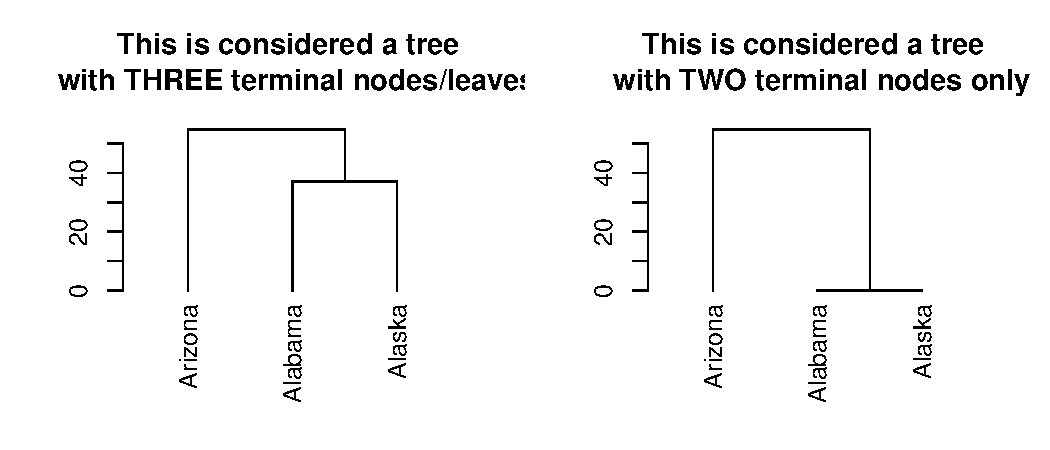
\includegraphics[width=\maxwidth]{figure/unnamed-chunk-19} 

}



\end{knitrout}



\section{Tree manipulation}

\subsection{Unrooting and root height}

A tree's nodes has various heights. Sometimes we are interested in changing the height of the entire tree. It is useful when This can be accomplished using \code{raise.dendrogram}. For example (notice how the entire tree's height is changed):

\begin{knitrout}
\definecolor{shadecolor}{rgb}{0.969, 0.969, 0.969}\color{fgcolor}\begin{kframe}
\begin{alltt}

hc <- \hlfunctioncall{hclust}(\hlfunctioncall{dist}(USArrests[1:3, ]), \hlstring{"ave"})
dend <- \hlfunctioncall{as.dendrogram}(hc)

taller_dend <- \hlfunctioncall{raise.dendrogram}(dend, 10)
shorter_dend <- \hlfunctioncall{raise.dendrogram}(dend, -10)

\hlfunctioncall{attr}(dend, \hlstring{"height"})  # 54.80041
\end{alltt}
\begin{verbatim}
## [1] 54.8
\end{verbatim}
\begin{alltt}
\hlfunctioncall{attr}(taller_dend, \hlstring{"height"})  # 64.80041
\end{alltt}
\begin{verbatim}
## [1] 64.8
\end{verbatim}
\begin{alltt}
\hlfunctioncall{attr}(shorter_dend, \hlstring{"height"})  # 44.80041
\end{alltt}
\begin{verbatim}
## [1] 44.8
\end{verbatim}
\begin{alltt}

\hlfunctioncall{par}(mfrow = \hlfunctioncall{c}(1, 3))
\hlfunctioncall{plot}(dend, ylim = \hlfunctioncall{c}(0, 70), main = \hlstring{"Original dend"})
\hlfunctioncall{abline}(h = \hlfunctioncall{c}(40, 50, 60), lty = 2)
\hlfunctioncall{plot}(taller_dend, ylim = \hlfunctioncall{c}(0, 70), main = \hlstring{"Taller dend"})
\hlfunctioncall{abline}(h = \hlfunctioncall{c}(40, 50, 60), lty = 2)
\hlfunctioncall{plot}(shorter_dend, ylim = \hlfunctioncall{c}(0, 70), main = \hlstring{"Shorter dend"})
\hlfunctioncall{abline}(h = \hlfunctioncall{c}(40, 50, 60), lty = 2)
\end{alltt}
\end{kframe}

{\centering 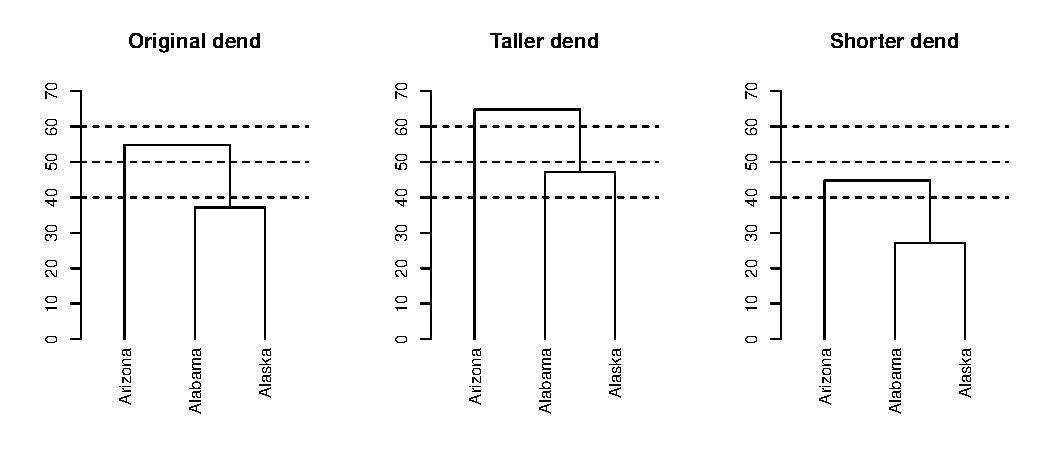
\includegraphics[width=\maxwidth]{figure/unnamed-chunk-20} 

}



\end{knitrout}




Sometimes we wish to "unroot" the dendrogram, meaning that we merge one of the tree's branches with its root. This is useful, for example, when merging phylogenetic trees from several families, and being unwilling to assume a specific root to the merged trees. Unrooting can be done using the \code{unroot} (S3) function (notice the use of the \code{branch_becoming_root} parameter):


\begin{knitrout}
\definecolor{shadecolor}{rgb}{0.969, 0.969, 0.969}\color{fgcolor}\begin{kframe}
\begin{alltt}

hc <- \hlfunctioncall{hclust}(\hlfunctioncall{dist}(USArrests[10:13, ]), \hlstring{"ward"})
dend <- \hlfunctioncall{as.dendrogram}(hc)

unrooted_dend <- \hlfunctioncall{unroot}(dend, branch_becoming_root = 1)
unrooted_dend_2 <- \hlfunctioncall{unroot}(unrooted_dend, branch_becoming_root = 3)

\hlfunctioncall{par}(mfrow = \hlfunctioncall{c}(1, 3))
\hlfunctioncall{plot}(dend)
\hlfunctioncall{plot}(unrooted_dend)
\hlfunctioncall{plot}(unrooted_dend_2)
\end{alltt}
\end{kframe}

{\centering 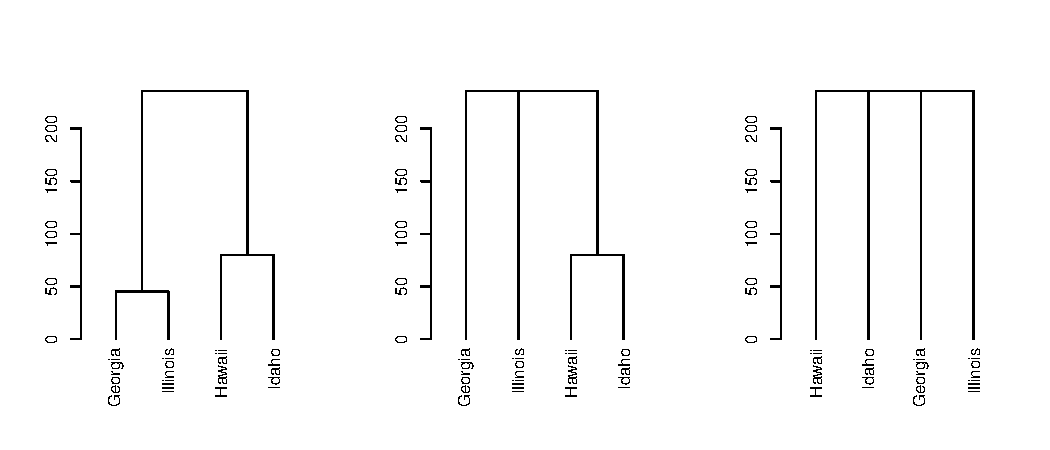
\includegraphics[width=\maxwidth]{figure/unnamed-chunk-21} 

}



\end{knitrout}


While the \code{unroot.hclust} method exists, it is not expected to work since \code{hclust} objects are not designed to handle non-binary trees (hence the advantage of using \code{dendrogram} objects). For \code{phylo} objects (from the \pkg{ape} package), there is also a method that would simply use \code{ape:::unroot(phy = x)}.

In some rare cases, we might wish to equalize the heights of root's branches. For this we can use the \code{flatten.dendrogram} function:


\begin{knitrout}
\definecolor{shadecolor}{rgb}{0.969, 0.969, 0.969}\color{fgcolor}\begin{kframe}
\begin{alltt}

hc <- \hlfunctioncall{hclust}(\hlfunctioncall{dist}(USArrests[10:13, ]), \hlstring{"ward"})
dend <- \hlfunctioncall{as.dendrogram}(hc)

flatten_dend_1 <- \hlfunctioncall{flatten.dendrogram}(dend, FUN = max)
flatten_dend_2 <- \hlfunctioncall{flatten.dendrogram}(dend, FUN = min)

\hlfunctioncall{par}(mfrow = \hlfunctioncall{c}(1, 3))
\hlfunctioncall{plot}(dend, main = \hlstring{"Original tree"})
\hlfunctioncall{abline}(h = \hlfunctioncall{c}(50, 100), lty = 2)
\hlfunctioncall{plot}(flatten_dend_1, main = \hlstring{"Flatten tree \textbackslash{}\hlfunctioncall{n}(max branches height)"})
\hlfunctioncall{abline}(h = \hlfunctioncall{c}(50, 100), lty = 2)
\hlfunctioncall{plot}(flatten_dend_2, main = \hlstring{"Flatten tree \textbackslash{}\hlfunctioncall{n}(min branches height)"})
\hlfunctioncall{abline}(h = \hlfunctioncall{c}(50, 100), lty = 2)
\end{alltt}
\end{kframe}

{\centering 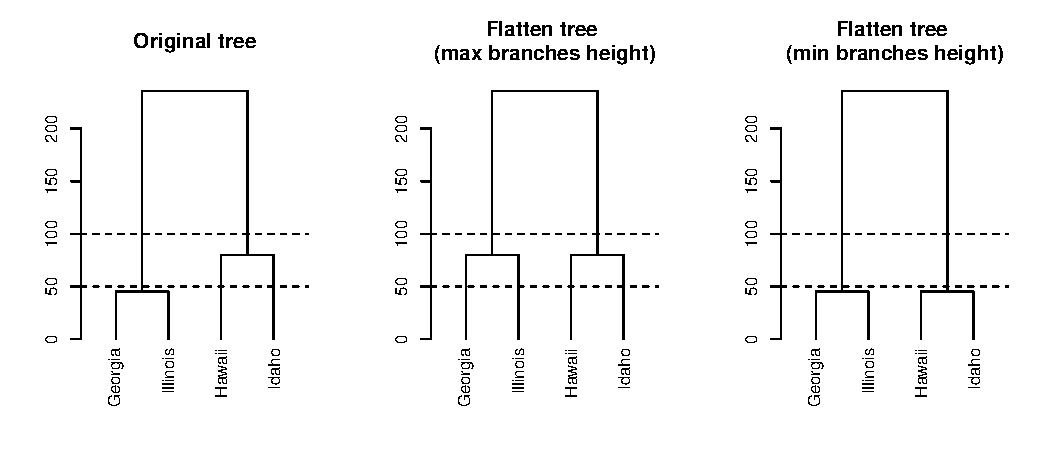
\includegraphics[width=\maxwidth]{figure/unnamed-chunk-22} 

}



\end{knitrout}





\subsection{Coloring labels of leaves}

Coloring labels can sometimes be useful, it is done through the \code{labels_colors} function (which also has assignemnt). Notice the assignment recycling, as well as the differene in the appearence of a dot when labels' color is black, compared to when it is NULL:

\begin{knitrout}
\definecolor{shadecolor}{rgb}{0.969, 0.969, 0.969}\color{fgcolor}\begin{kframe}
\begin{alltt}

\hlfunctioncall{par}(mfrow = \hlfunctioncall{c}(1, 3))

hc <- \hlfunctioncall{hclust}(\hlfunctioncall{dist}(USArrests[1:3, ]), \hlstring{"ave"})
dend <- \hlfunctioncall{as.dendrogram}(hc)

\hlcomment{# Defaults:}
\hlfunctioncall{labels_colors}(dend)
\end{alltt}
\begin{verbatim}
## NULL
\end{verbatim}
\begin{alltt}
\hlfunctioncall{plot}(dend)

\hlcomment{# let's add some color:}
\hlfunctioncall{require}(colorspace)
\end{alltt}


{\ttfamily\noindent\itshape\color{messagecolor}{\#\# Loading required package: colorspace}}\begin{alltt}
\hlfunctioncall{labels_colors}(dend) <- \hlfunctioncall{rainbow_hcl}(3)
\hlfunctioncall{labels_colors}(dend)
\end{alltt}
\begin{verbatim}
##   Arizona   Alabama    Alaska 
## "#E495A5" "#86B875" "#7DB0DD"
\end{verbatim}
\begin{alltt}
\hlfunctioncall{plot}(dend)

\hlcomment{# changing color to black}
\hlfunctioncall{labels_colors}(dend) <- 1
\end{alltt}


{\ttfamily\noindent\color{warningcolor}{\#\# Warning: Length of color vector was shorter then the number of leaves - vector color recycled}}\begin{alltt}
\hlfunctioncall{labels_colors}(dend)
\end{alltt}
\begin{verbatim}
## Arizona Alabama  Alaska 
##       1       1       1
\end{verbatim}
\begin{alltt}
\hlfunctioncall{plot}(dend)
\end{alltt}
\end{kframe}

{\centering 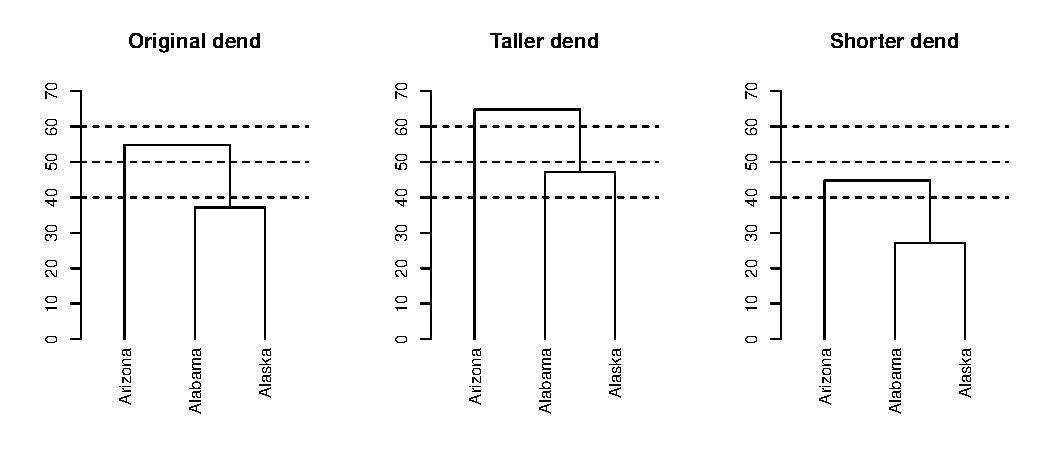
\includegraphics[width=\maxwidth]{figure/unnamed-chunk-23} 

}


\begin{kframe}\begin{alltt}

\hlcomment{# removing color (and the nodePar completely - if it has no other}
\hlcomment{# attributed but lab.col)}
\hlfunctioncall{labels_colors}(dend) <- NULL
\end{alltt}


{\ttfamily\noindent\color{warningcolor}{\#\# Warning: Length of color vector was shorter then the number of leaves - vector color recycled}}

{\ttfamily\noindent\color{warningcolor}{\#\# Warning: 'x' is NULL so the result will be NULL}}\begin{alltt}
\hlfunctioncall{labels_colors}(dend)
\end{alltt}
\begin{verbatim}
## NULL
\end{verbatim}
\end{kframe}
\end{knitrout}




\subsection{Trimming leaves}

Trimming a tree from some leaves can be done using the \code{trim} (S3 method) function (notice that the attributes of the trimmed tree are updated):

\begin{knitrout}
\definecolor{shadecolor}{rgb}{0.969, 0.969, 0.969}\color{fgcolor}\begin{kframe}
\begin{alltt}

hc <- \hlfunctioncall{hclust}(\hlfunctioncall{dist}(USArrests[1:5, ]), \hlstring{"ave"})
dend <- \hlfunctioncall{as.dendrogram}(hc)
\hlfunctioncall{library}(colorspace)
\hlfunctioncall{labels_colors}(dend) <- \hlfunctioncall{rainbow_hcl}(5)

trimmed_dend <- \hlfunctioncall{trim}(dend, \hlfunctioncall{c}(\hlstring{"Alaska"}, \hlstring{"California"}))

\hlfunctioncall{str}(\hlfunctioncall{unclass}(trimmed_dend))
\end{alltt}
\begin{verbatim}
## List of 2
##  $ : atomic [1:1] 4
##   ..- attr(*, "members")= int 1
##   ..- attr(*, "height")= num 0
##   ..- attr(*, "label")= chr "Arkansas"
##   ..- attr(*, "leaf")= logi TRUE
##   ..- attr(*, "nodePar")=List of 1
##   .. ..$ lab.col: chr "#E495A5"
##  $ :List of 2
##   ..$ : atomic [1:1] 3
##   .. ..- attr(*, "label")= chr "Arizona"
##   .. ..- attr(*, "members")= int 1
##   .. ..- attr(*, "height")= num 0
##   .. ..- attr(*, "leaf")= logi TRUE
##   .. ..- attr(*, "nodePar")=List of 1
##   .. .. ..$ lab.col: chr "#BDAB66"
##   ..$ : atomic [1:1] 1
##   .. ..- attr(*, "label")= chr "Alabama"
##   .. ..- attr(*, "members")= int 1
##   .. ..- attr(*, "height")= num 0
##   .. ..- attr(*, "leaf")= logi TRUE
##   .. ..- attr(*, "nodePar")=List of 1
##   .. .. ..$ lab.col: chr "#55B8D0"
##   ..- attr(*, "members")= num 2
##   ..- attr(*, "midpoint")= num 0.5
##   ..- attr(*, "height")= num 52.6
##  - attr(*, "members")= num 3
##  - attr(*, "midpoint")= num 0.75
##  - attr(*, "height")= num 82.6
\end{verbatim}
\begin{alltt}

\hlfunctioncall{par}(mfrow = \hlfunctioncall{c}(1, 2))
\hlfunctioncall{plot}(dend, main = \hlstring{"Original tree"})
\hlfunctioncall{plot}(trimmed_dend, main = \hlstring{"Tree without Alaska and California"})
\end{alltt}
\end{kframe}

{\centering 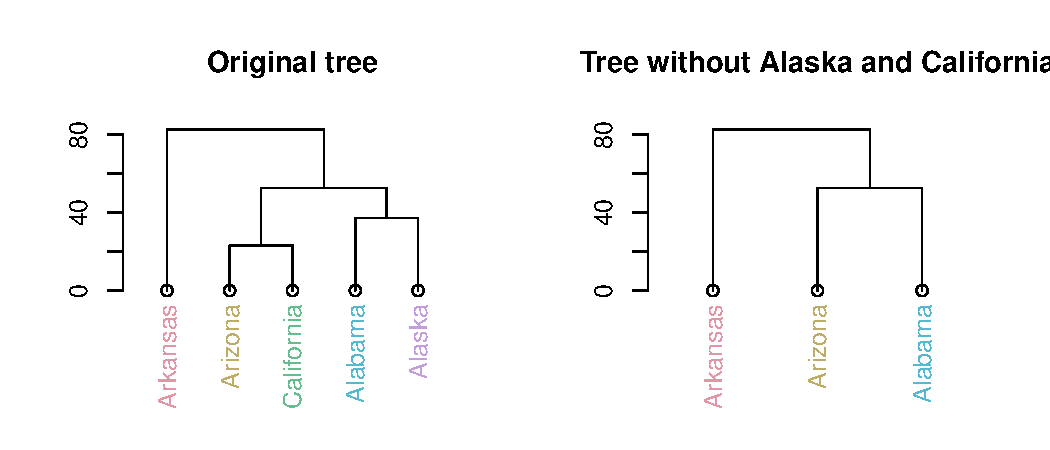
\includegraphics[width=\maxwidth]{figure/unnamed-chunk-24} 

}



\end{knitrout}


If we have two trees, we can use the \code{intersect_trees} function to reduce both trees to have the same labels (this will be useful later when we'd like to compare the two trees):


\begin{knitrout}
\definecolor{shadecolor}{rgb}{0.969, 0.969, 0.969}\color{fgcolor}\begin{kframe}
\begin{alltt}

hc_1 <- \hlfunctioncall{hclust}(\hlfunctioncall{dist}(USArrests[1:5, ]), \hlstring{"single"})
hc_2 <- \hlfunctioncall{hclust}(\hlfunctioncall{dist}(USArrests[1:5, ]), \hlstring{"complete"})
dend_1 <- \hlfunctioncall{as.dendrogram}(hc_1)
dend_2 <- \hlfunctioncall{as.dendrogram}(hc_2)

\hlfunctioncall{library}(colorspace)
\hlfunctioncall{labels_colors}(dend_1) <- \hlfunctioncall{rainbow_hcl}(5)
\hlfunctioncall{labels_colors}(dend_2) <- \hlfunctioncall{rainbow_hcl}(5)


trimmed_dend_1 <- \hlfunctioncall{trim}(dend_1, \hlfunctioncall{c}(\hlstring{"Alaska"}))
trimmed_dend_2 <- \hlfunctioncall{trim}(dend_2, \hlfunctioncall{c}(\hlstring{"California"}))

dends_12 <- \hlfunctioncall{intersect_trees}(trimmed_dend_1, trimmed_dend_2)

\hlfunctioncall{par}(mfrow = \hlfunctioncall{c}(3, 2))
\hlfunctioncall{plot}(dend_1, main = \hlstring{"Tree - single method"}, ylim = \hlfunctioncall{c}(0, 110))
\hlfunctioncall{plot}(dend_2, main = \hlstring{"Tree - complete method"}, ylim = \hlfunctioncall{c}(0, 110))
\hlfunctioncall{plot}(trimmed_dend_1, main = \hlstring{"Trimmed tree - single method"}, ylim = \hlfunctioncall{c}(0, 110))
\hlfunctioncall{plot}(trimmed_dend_2, main = \hlstring{"Trimmed tree - complete method"}, ylim = \hlfunctioncall{c}(0, 110))
\hlfunctioncall{plot}(dends_12[[1]], main = \hlstring{"Intersected tree - single method"}, ylim = \hlfunctioncall{c}(0, 110))
\hlfunctioncall{plot}(dends_12[[2]], main = \hlstring{"Intersected tree - complete method"}, ylim = \hlfunctioncall{c}(0, 
    110))
\end{alltt}
\end{kframe}

{\centering 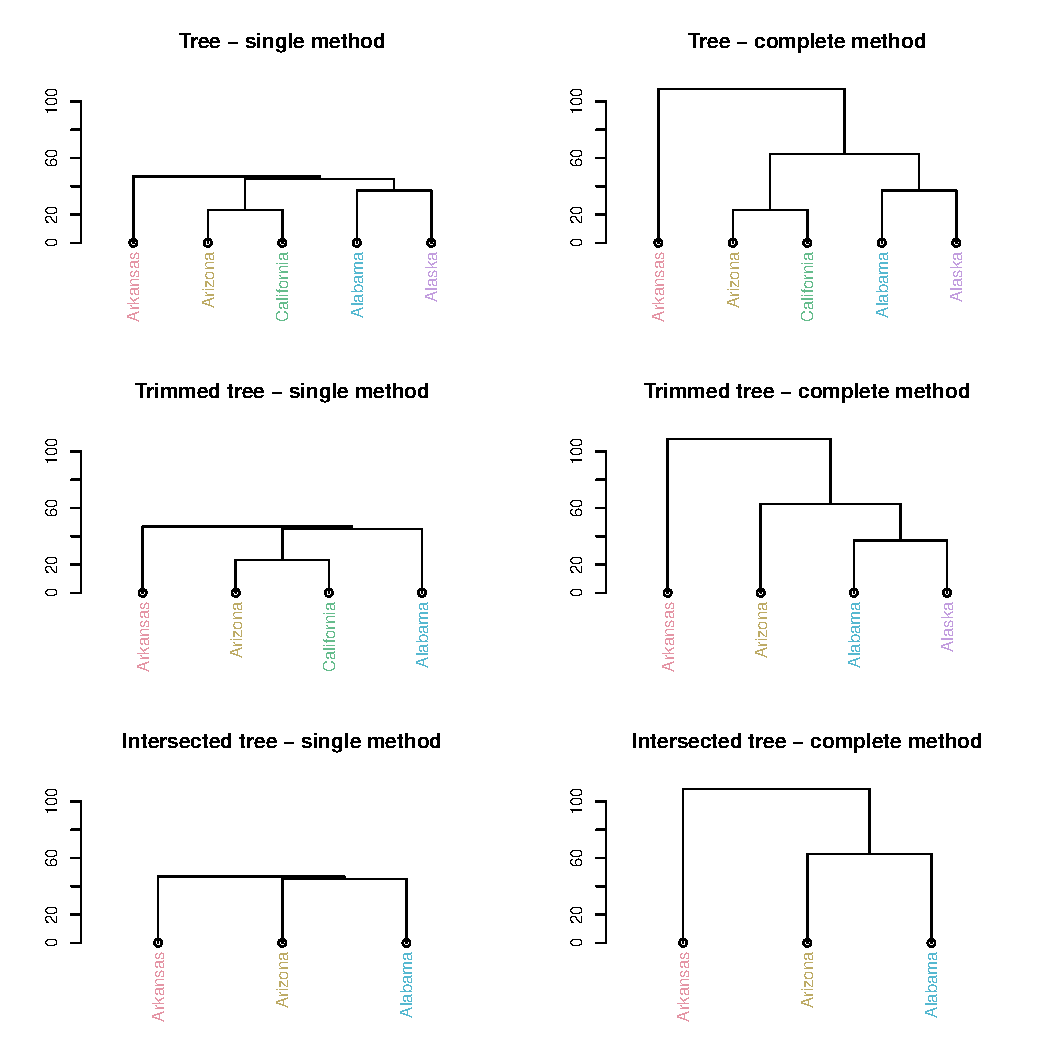
\includegraphics[width=\maxwidth]{figure/unnamed-chunk-25} 

}


\begin{kframe}\begin{alltt}


\end{alltt}
\end{kframe}
\end{knitrout}


Sidenote: a similar function, called \code{plotColoredClusters}, is available in the \pkg{ClassDiscovery} package for \code{hclust} objects.


\subsection{Rotating branches}

A dendrogram is an object which can be rotated on its hinges without 
changing its topological.

Rotating a dendrogram in base R can be done using the \code{reorder} function.
The problem with this function is that it is not very intuitive. For this reason
we wrote the \code{rotate} function. It has two main arguments: the object, and
the order we wish to rotate it by. The order parameter can be either a numeric
vector, used in a similar way we would order a simple character vector. Or, the
order parameter can also be a character vector of the labels of the tree, given
in the new desired order of the tree.

It is also worth noting that some order are impossible to achieve for a given 
tree's topology. In such a case, the function will do its "best" to get as close
as possible.

Here are a few examples:


\begin{knitrout}
\definecolor{shadecolor}{rgb}{0.969, 0.969, 0.969}\color{fgcolor}\begin{kframe}
\begin{alltt}

hc <- \hlfunctioncall{hclust}(\hlfunctioncall{dist}(USArrests[\hlfunctioncall{c}(1, 6, 13, 20, 23), ]), \hlstring{"ave"})
dend <- \hlfunctioncall{as.dendrogram}(hc)

\hlcomment{# For dendrogram objects:}
\hlfunctioncall{require}(colorspace)
\hlfunctioncall{labels_colors}(dend) <- \hlfunctioncall{rainbow_hcl}(\hlfunctioncall{nleaves}(dend))
\hlcomment{# let's color the labels to make the followup of the rotation easier}
\hlfunctioncall{par}(mfrow = \hlfunctioncall{c}(2, 2))
\hlfunctioncall{plot}(dend, main = \hlstring{"Original tree"})
\hlfunctioncall{plot}(\hlfunctioncall{rotate}(dend, \hlfunctioncall{c}(2:5, 1)), main = \hlstring{"Rotates the left most leaf \textbackslash{}n into the right side of the tree"})
\hlfunctioncall{plot}(dend, main = \hlstring{"Original tree"})
\hlfunctioncall{plot}(\hlfunctioncall{sort}(dend), main = \hlstring{"Sorts the labels by alphabetical order \textbackslash{}n\textbackslash{}nand rotates the tree to give the best fit possible"})
\end{alltt}
\end{kframe}

{\centering 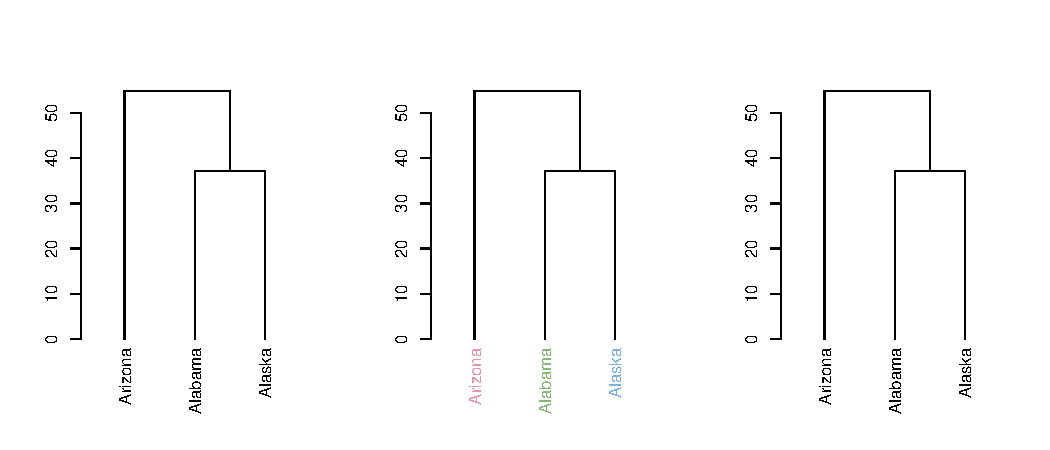
\includegraphics[width=\maxwidth]{figure/unnamed-chunk-26} 

}



\end{knitrout}







\subsection{Coloring branches}


Dendrogram plots with colored branches have been available in R for many years in threads on the mailing lists and through various package. However, until recently, all of the functions in packages have always given the user a new \code{plot} function, without seperating the coloring of branches of a dendrogram from its plotting. Often the function for actually plotting the colored branched dendrogram would be hidden from the user. For example, the \pkg{labeltodendro} package \citep{CRAN:labeltodendro} gives a colored branch plot through the \code{colorplot} function, but the work horse for this is available in a hidden function called \code{dendroploth} or \code{dendroplotv}, both take care of the plotting by themselves (instead of modifying the dendrogram object, and then letting the base R function do the work). The same story happens in the \pkg{Heatplus} \citep{CRAN:Heatplus}, where the \code{plot.annHeatmap2} function actually uses the hidden function \code{cutplot.dendrogram} for doing the plotting.

This was changed in the beginning of 2013 thanks to Gregory Jefferis's \pkg{dendroextras} package \citep{CRAN:dendroextras}, which orgranized this through the \code{colour_clusters} function. In the \pkg{dendextend} package I will mostly import his code, with some modifications. The biggest limitation in Gregory's code is that he relies on changing the \code{dendrogram} into \code{hclust} in order to use \code{cutree} on it and get the clusters. This has the advantage of being fast, but the \textbf{disadvantage} that it restricts his code to binary trees only. For this reason, I will not use his \code{slice} function, and made sure to use other functions instead.






\section{Tanglegrams - visually comparing two trees side-by-side}

\subsection{Tanglegram visualization}

\subsection{Finding an optimal rotation}


\section{Comparing two trees - statistics and inference}

\subsection{Baker's gamma}

\subsection{Bk method}














% 
% 
% a short review of other approaches and give some historical
% background on the development of \pkg{dendextend}.
% 
% 
% Several examples are included to illustrate the functionality of \pkg{dendextend}. Many more examples are available within
% the package. % , both as explicit examples and as part of the numerous unit tests.
% %
% The \pkg{dendextend} package is available from the Comprehensive \proglang{R} Archive Network (CRAN)
% at \url{http://CRAN.R-project.org/package=dendextend}.
% 
% \makeatletter
% \if@nojss
%   This vignette will one day corresponds to a paper 
%   
% %   published in the \textsl{Journal of Statistical Software}. It is currently still identical to the published paper.  
%   
%   Over time, this vignette version may receive minor
%   updates. For citations, please use %the \cite{JSS:dendextend} or
%   % \cite{Eddelbuettel:2013:dendextend}; details are also provided in
%   \proglang{R} via \texttt{citation("dendextend")}.
% 
%   This version corresponds to \pkg{dendextend} version dendextend.version and was typeset on now.date.
% \fi
% \makeatother
% 

% \subsection{Historical context}
% \subsection{Related work}

%%% \cite - name and date in (),, \citep - (all in ())
% \cite{TempleLang:2009:RGCCTranslationUnit}, 

% \subsection[dendextend use cases]{\pkg{dendextend} use cases}
% \label{sec:classic_dendextend}

% \subsection[dendextend class hierarchy]{\pkg{dendextend} class hierarchy}
% \subsection{Derived classes}

% \subsection{Character vectors}

% \section[R and C++ data interchange]{\proglang{R} and \proglang{C++} data interchange}

% \subsection[C++ to R: wrap]{\proglang{C++} to \proglang{R}: \code{wrap}}
% \subsection[R to C++: as]{\proglang{R} to \proglang{C++}: \code{as}}

% The \citep command is used where the author name is to appear inside the parentheses alongside the date.
% \citep{Sanderson:2010:Armadillo}.


% \subsection{Implicit use of converters}

% \section{Function calls}
% \label{sec:functions}

% \section{Using code `inline'}
% \label{sec:inline}
% \code{update.packages()} 
% \footnote{This presumes a platform for which pre-built binaries are}
% \cite{CRAN:dendextend:Attributes} for more details.

% \section{Using Standard Template Library algorithms}

% \citep{Plauger+Et+Al:2000:STL}. 


% \section{Error handling}
% \subsection[C++ exceptions in R]{\proglang{C++} exceptions in \proglang{R}}
% \subsection[R errors in C++]{\proglang{R} errors in \proglang{C++}}


% \section{Performance comparison}
% \label{sec:perfcomp}



% %
% \begin{Code}
% ...
% \end{Code}
% %

% are summarized in Table~\ref{tab:benchmark} below.
% 
% \begin{table}[t]
%   \begin{center}
%     \begin{small}
%       \begin{tabular}{lrr}
%         \toprule
%         Implementation                    & Time in millisec. & Relative to \proglang{R} API \\
%         \cmidrule(r){2-3}
%         \proglang{R} API (as benchmark)             &  218       & \\
%         \pkg{dendextend} sugar                        &  145       & 0.67 \\
%         \code{NumericVector::iterator}    &  217       & 1.00 \\
%         \code{NumericVector::operator[]}  &  282       & 1.29 \\
%         %\code{dendextendVector<double>}         &  683       & 3.13 \\
%         \bottomrule
%       \end{tabular}
%     \end{small}
%     \caption{Run-time performance of the different convolution examples.}
%     \label{tab:benchmark}
%   \end{center}
% \end{table}
% 

% \section{On-going development}
% \label{sec:ongoing}

% \code{head},


\section{Summary}

The \pkg{dendextend} package presented in this paper greatly extends the available functionality of the dendrogram objects in \proglang{R}.

% compiled \proglang{C++} code with \proglang{R}.
% \pkg{dendextend} provides a \proglang{C++} class hierarchy which allows manipulation of \proglang{R} data structures in \proglang{C++}
% using member functions and operators directly related to the type
% of object being used, thereby reducing the level of expertise
% required to master the various functions and macros offered by the
% internal \proglang{R} API. The classes assume the entire
% responsibility of garbage collection of objects, relieving the
% programmer from book-keeping operations with the protection stack
% and enabling him/her to focus on the underlying problem.
% 
% Data interchange between \proglang{R} and \proglang{C++} code is performed by the \code{wrap()} and
% \code{as()} template functions. They allow the programmer to write logic in terms
% of \proglang{C++} data structures, and facilitate use of modern libraries such as the
% Standard Template Library (STL) and its containers and algorithms. The
% \code{wrap()} and \code{as()} template functions are extensible by
% design. They are also used either explicitly or implicitly throughout the API.
% By using only thin wrappers around \code{SEXP} objects and adopting \proglang{C++}
% idioms such as iterators, the footprint of the \pkg{dendextend} API
% is very lightweight, and does not incur a significant performance penalty.
% 
% The \pkg{dendextend} API offers opportunities to dramatically reduce the complexity
% of code, which should lower the initial cost of writing code and improve code readability, maintainability, and
% reuse---without incurring noticeable penalties in run-time performance.



\section*{Acknowledgments}

We are very thankful for code contributions and ideas by the R core team (especially Martin Maechler and Brian Ripley, but probably also others without our knowledge), Gavin Simpson, Gregory Jefferis
,
% Detailed comments and suggestions by editors as well as anonymous referees
% are gratefully acknowledged.  




\bibliography{dendextend-tutorial}

\vspace*{-0.35cm}

\end{document}

%%% Local Variables:
%%% mode: latex
%%% TeX-master: t
%%% End:


%% library(knitr)
%% Sweave2knitr('vignettes\\dendextend-tutorial.rnw')
